% !TEX program = pdflatex
\documentclass[11pt,a4paper]{amsart}

% --- ENCODING & FONTS ------------------------------------------------------
\usepackage[utf8]{inputenc}
\usepackage[T1]{fontenc}

% --- MATH PACKAGES ---------------------------------------------------------
\usepackage{amsmath,amssymb,amsthm,mathtools}
\usepackage{graphicx}

% --- PAGE LAYOUT -----------------------------------------------------------
\usepackage{geometry}
\geometry{a4paper,left=25mm,right=25mm,top=25mm,bottom=30mm}

% --- HYPERLINKS ------------------------------------------------------------
\usepackage[hyphens]{url}
\usepackage[colorlinks=true, urlcolor=blue, linkcolor=blue]{hyperref}
\usepackage{doi}

\hypersetup{
    pdftitle={An Analytic Prime Indicator Based on the Fejér Kernel},
    pdfauthor={Sebastian Fuchs (ORCID: 0009-0009-1237-4804)},
    pdfkeywords={Prime numbers, analytic prime indicator, analytic number theory, trigonometric series, Fejér kernel, sebastian.fuchs@hu-berlin.de},
    pdfsubject={Primary 11A41; Secondary 11L03, 42A10}
}

% --- MACROS & THEOREMS -----------------------------------------------------
\newcommand{\Px}{\mathcal{P}}
\newcommand{\R}{\mathbb{R}}

% --- THEOREM STYLES --------------------------------------------------------
\theoremstyle{plain}
\newtheorem{theorem}{Theorem}[section]
\newtheorem{conjecture}[theorem]{Conjecture}
\newtheorem{lemma}[theorem]{Lemma}
\newtheorem{property}[theorem]{Property}
\theoremstyle{definition}
\newtheorem{definition}[theorem]{Definition}


% --- METADATA --------------------------------------------------------------
\title[An Analytic Prime Indicator]{An Analytic Prime Indicator Based on the Fejér Kernel\thanks{To cite this work, please use the permanent identifier (DOI): \doi{10.5281/zenodo.15712807}}}
\author{Sebastian Fuchs}
\address{Institut für Mathematik, Humboldt-Universität zu Berlin, 10099 Berlin, Germany}
\email{sebastian.fuchs@hu-berlin.de}
\urladdr{https://orcid.org/0009-0009-1237-4804}
\date{June 22, 2025}
\subjclass[2020]{Primary 11A41; Secondary 11L03, 42A10}
\keywords{Prime numbers, analytic prime indicator, analytic number theory, trigonometric series, Fejér kernel}

% ---------------------------------------------------------------------------
\begin{document}

\begin{abstract}
This note introduces an analytic prime indicator, constructed by smoothing a trigonometric analogue of trial division. First, a function $\Px\colon\R\to\R$ of class $C^1$ is presented, whose zeros for $x>2$ correspond precisely to the odd primes. Its second derivative exhibits jump discontinuities at integer squares. Subsequently, it is shown how this construction can be modified via an infinite series to yield a globally smooth function, $\Px_{\phi}$, of class $C^\infty$ that preserves this prime-zero property. As a primary application, it is demonstrated how this indicator can be used to construct an analytic approximation for the prime-counting function $\pi(x)$ with a provably controlled error.
\end{abstract}

\maketitle

% ---------------------------------------------------------------------------
\section{Introduction}
Prime numbers occupy a central position in number theory, and explicit functions that identify primes have long been a subject of fascination~\cite{hardy2008}. Early celebrated results include the non-constructive formula of Mills, which relies on the existence of a special constant~\cite{mills1947}, and the explicit but computationally infeasible formula of Willans, which is based on Wilson's theorem~\cite{willans1964}.
The quest for such functions remains a vibrant area of research. Modern approaches are diverse, ranging from purely arithmetic constructions~\cite{mazzanti2024} to various forms of analytic indicators~\cite{helfgott2023, hiary2018, seriprim2022}. A recent focus has been the development of smooth, differentiable functions that approximate the characteristic function of the primes, for instance through integral kernel methods~\cite{semenov2025}.

In this note, a new type of analytic prime indicator, $\Px(x)$, is introduced, contributing to this line of inquiry. The method presented here differs from previous approaches in that it is based on the principles of Fourier analysis. Specifically, $\Px(x)$ is constructed by regularising a trigonometric representation of trial division using the Fejér kernel, a classical tool for ensuring the convergence of trigonometric series~\cite{zygmund2002}.
This paper establishes the function's basic analytic properties, proves its "prime-zero property", and shows how it can be modified to yield a globally smooth function $\Px_{\phi}(x)$ of class $C^\infty$ that preserves this core property. A key application of this framework is the construction of an approximation for the prime-counting function $\pi(x)$ with a provably controlled error. Throughout, $\lceil t \rceil$ denotes the ceiling of a real number~$t$.

% ---------------------------------------------------------------------------
\section{Analytic construction of $\Px$}

\subsection{Motivation}\label{subsec:motivation}
Trial division classifies an integer $x$ as composite once an integer divisor $i\le\sqrt{x}$ is found. Analytically, the quotient
\[
Q(x,i)=\frac{\sin^{2}(\pi x)}{\sin^{2}(\pi x/i)}
\]
vanishes for integer~$x$ whenever $i\nmid x$ and is undefined when $i\mid x$.
\subsection{Regularisation}
Invoking the Fejér identity
\[
\frac{\sin^{2}(ny)}{\sin^{2}y}=n+2\sum_{k=1}^{n-1}(n-k)\cos(2ky)
\]
with $n=i$ and $y=\pi x/i$ removes the indeterminacy and yields a finite cosine sum that extends $Q$ to real~$x$.

\subsection{Definition}
\begin{definition}\label{def:Px}
For $x>1$ define
\begin{equation}\label{eq:Px}
\Px(x)=\frac{1}{x}\sum_{i=2}^{\lceil\sqrt{x}\rceil}\left(i+2\sum_{k=1}^{i-1}(i-k)\cos\left(\frac{2\pi k x}{i}\right)\right),
\end{equation}
and set $\Px(x)=0$ for $x\le1$.
\end{definition}

% ---------------------------------------------------------------------------
\section{Smoothness properties of $\Px$}

\subsection{Global $C^{1}$-smoothness}
\begin{property}\label{prop:C1}
The function $\Px$ is continuous on $\R$ and of class $C^1$ for $x>0$.
\end{property}
\begin{proof}
Let $F(x,i)$ denote the term in the summation in Definition~\ref{def:Px}. On any open interval $((m-1)^2, m^2)$ for $m\ge 2$, the summation limit $\lceil\sqrt{x}\rceil$ is fixed at $m$, making $\Px$ a finite sum of $C^\infty$ functions and thus $C^\infty$ on these intervals. The critical points are the integer squares $x=m^2$, where the limit jumps from $m$ to $m+1$.
First, continuity at $x=m^2$ is established. As $x \to (m^2)^-$, the function is $\Px(x) = \frac{1}{x}\sum_{i=2}^{m} F(x,i)$. As $x \to (m^2)^+$, an additional term $\frac{1}{x}F(x,m+1)$ appears. Continuity requires this new term to be zero at the transition point.
At $x=m^2$, the argument of the cosine in $F(m^2, m+1)$ becomes $\frac{2\pi k m^2}{m+1} = 2\pi k(m-1) + \frac{2\pi k}{m+1}$. Thus,
\[ F(m^2, m+1) = (m+1) + 2\sum_{k=1}^{m}(m+1-k)\cos\left(\frac{2\pi k}{m+1}\right). \]
This is the Fejér kernel $K_m(t)$ evaluated at $t=2\pi/(m+1)$, which equals $\frac{\sin^2((m+1)t/2)}{\sin^2(t/2)} = \frac{\sin^2(\pi)}{\sin^2(\pi/(m+1))} = 0$ for $m \ge 1$. The added term $\frac{1}{m^2}F(m^2, m+1)$ is zero, proving continuity.

Next, $C^1$-smoothness is established. The derivative $\Px'(x)$ exists on the open intervals. For $\Px$ to be of class $C^1$ at $x=m^2$, equality of the left-sided and right-sided limits of $\Px'(x)$ is required. This is equivalent to showing that the derivative of the newly added term, $\frac{d}{dx}\left[\frac{1}{x}F(x, m+1)\right]$, vanishes at $x=m^2$.
By the quotient rule, this derivative is $\frac{x F'(x, m+1) - F(x, m+1)}{x^2}$. Since $F(m^2, m+1)=0$, it is only necessary to show that $F'(m^2, m+1)=0$, where the derivative is with respect to $x$.
The derivative with respect to $x$ is:
\[ F'(x, i) = \frac{\partial}{\partial x}\left[i+2\sum_{k=1}^{i-1}(i-k)\cos\left(\frac{2\pi k x}{i}\right)\right] = -\frac{4\pi}{i}\sum_{k=1}^{i-1}k(i-k)\sin\left(\frac{2\pi k x}{i}\right). \]
Evaluating at $x=m^2$ and $i=m+1$:
\[ F'(m^2, m+1) = -\frac{4\pi}{m+1}\sum_{k=1}^{m}k(m+1-k)\sin\left(\frac{2\pi k m^2}{m+1}\right). \]
Using $\frac{m^2}{m+1} = m-1 + \frac{1}{m+1}$, the sine term becomes $\sin\left(2\pi k(m-1) + \frac{2\pi k}{m+1}\right) = \sin\left(\frac{2\pi k}{m+1}\right)$. The sum is
\[ S = \sum_{k=1}^{m}k(m+1-k)\sin\left(\frac{2\pi k}{m+1}\right). \]
The sum $S$ vanishes due to the symmetry of its terms. Specifically, the $k$-th and $(m+1-k)$-th terms cancel each other out, since for $j=m+1-k$, the $j$-th term is:
\begin{align*}
(m+1-k)(k)\sin\left(\frac{2\pi (m+1-k)}{m+1}\right) &= k(m+1-k)\sin\left(2\pi - \frac{2\pi k}{m+1}\right) \\
&= -k(m+1-k)\sin\left(\frac{2\pi k}{m+1}\right).
\end{align*}
If $m+1$ is odd, all terms pair up and cancel. If $m+1$ is even, say $m+1=2N$, there is a middle term for $k=N$, which is $N(2N-N)\sin\left(\frac{2\pi N}{2N}\right) = N^2\sin(\pi) = 0$. In all cases, the sum $S=0$.
Thus, $F'(m^2, m+1) = 0$, which ensures the derivative is continuous across the integer squares.
\end{proof}

\subsection{Second-derivative jumps}
\begin{property}\label{prop:second}
$\Px''$ has jump discontinuities at each integer square $x=m^2$, for $m\ge2$.
\end{property}
\begin{proof}
The jump is caused by the second derivative of the term $\frac{1}{x}F(x, m+1)$, which is added to the definition of $\Px(x)$ as $x$ crosses $m^2$. Since the term itself and its first derivative are zero at $x=m^2$, the magnitude of the jump in $\Px''(x)$ is precisely the value of this term's second derivative at that point.
A calculation shows that $\frac{d^2}{dx^2}\left[\frac{F(x,m+1)}{x}\right]_{x=m^2} = \frac{F''(m^2, m+1)}{m^2}$. The second derivative of the Fejér term is $F''(x, i) = -\frac{8\pi^2}{i^2}\sum_{k=1}^{i-1}k^2(i-k)\cos\left(\frac{2\pi k x}{i}\right)$.
At $x=m^2$ and $i=m+1$, this becomes $F''(m^2, m+1) = -\frac{8\pi^2}{(m+1)^2}\sum_{k=1}^{m}k^2(m+1-k)\cos\left(\frac{2\pi k}{m+1}\right)$, which is in general non-zero.
For instance, for $m=2$ (the jump at $x=4$), a direct calculation yields $F''(4, 3) = -\frac{8\pi^2}{9} \sum_{k=1}^{2}k^2(3-k)\cos\left(\frac{2\pi k}{3}\right) = -\frac{8\pi^2}{9}(1^2\cdot 2 \cdot (-\frac{1}{2}) + 2^2\cdot 1 \cdot (-\frac{1}{2})) = \frac{8\pi^2}{3} \neq 0$.
This non-vanishing contribution causes the jump discontinuity, which is a direct consequence of the sharp cutoff in the summation at $i = \lceil\sqrt{x}\rceil$.
\end{proof}

\begin{figure}[!htbp]
\centering
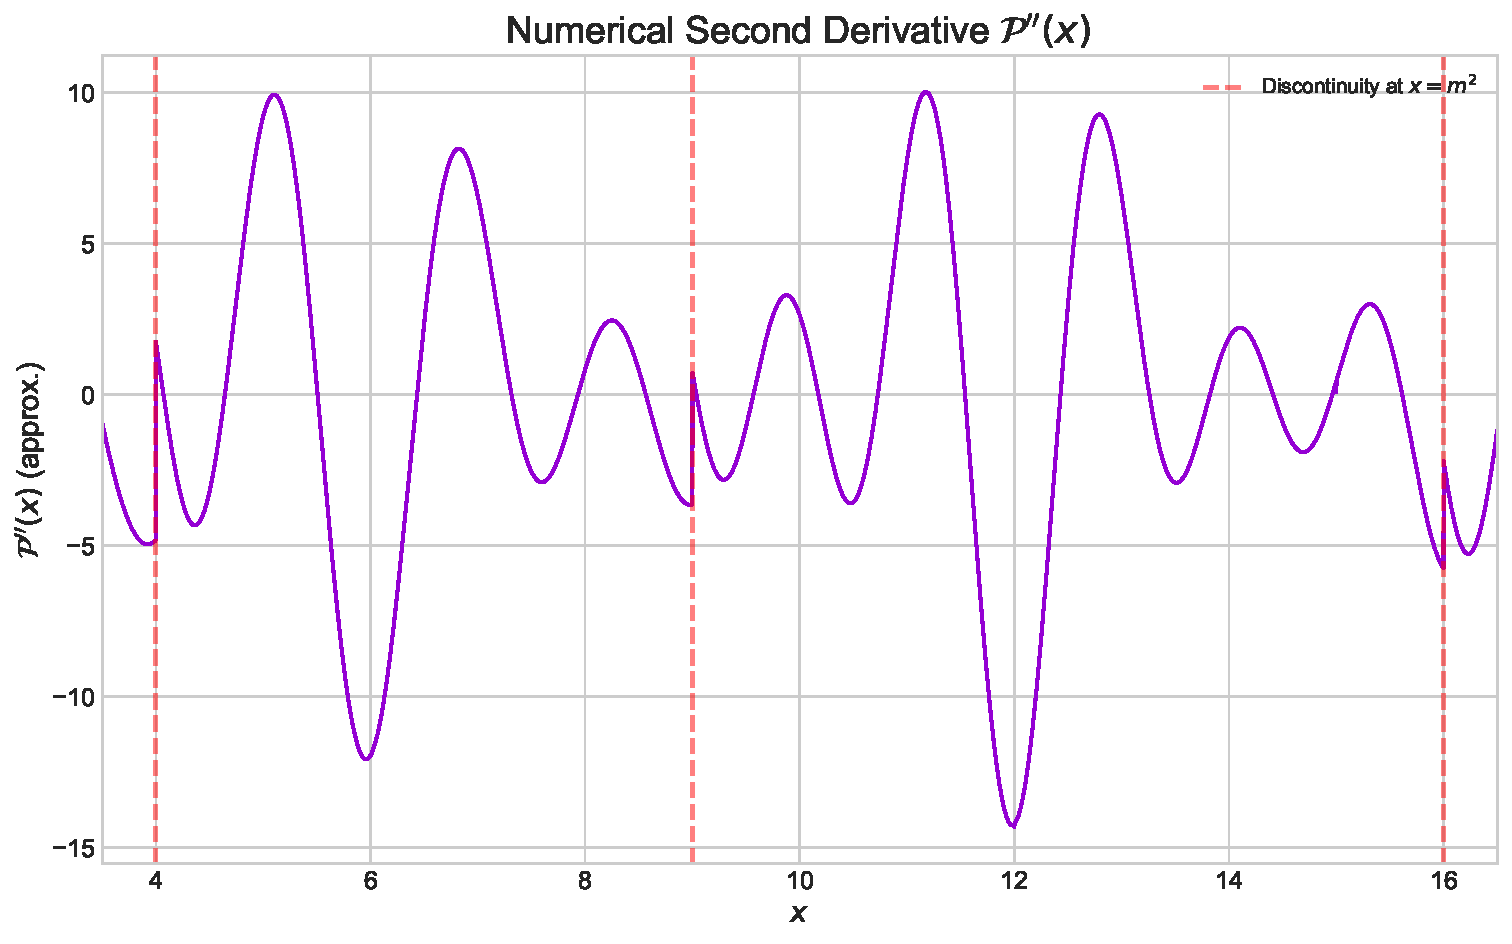
\includegraphics[width=\textwidth]{plot_second_derivative.pdf}
\caption{Finite-difference approximation of $\Px''(x)$ on $[3.5,16.5]$. Jump discontinuities are visible at $x=4,9,16$ (integer squares), in agreement with Property~\ref{prop:second}.}
\label{fig:secondderivative}
\end{figure}

% ---------------------------------------------------------------------------
\section{The Prime-Zero Property}

The main result of this note establishes that the function $\Px(x)$ acts as an indicator for odd prime numbers. This property is formalized in the following theorem.

\begin{theorem}[Prime-Zero Property]\label{thm:primezero}
For all real $x>2$, the function $\Px(x)$ has the property
\[
\Px(x)=0 \quad\Longleftrightarrow\quad x \text{ is an odd prime}.
\]
Furthermore, for all non-prime $x>2$, $\Px(x) > 0$.
\end{theorem}

\begin{proof}
The property is proven by considering three exhaustive cases for $x > 2$. Let $F(x,i)$ denote the term within the main summation in Definition~\ref{def:Px}.
\begin{enumerate}
  \item \textbf{Case 1: Let $x = p$, where $p$ is an odd prime.}
  The sum for $\Px(p)$ runs from $i=2$ to $\lceil\sqrt{p}\rceil$. For any integer $i$ in this range, by the definition of a prime number, $i$ is not a divisor of $p$. The term $F(p, i)$ is thus given by the non-singular form of the Fejér kernel, $F(p, i) = \frac{\sin^2(\pi p)}{\sin^2(\pi p/i)}$. Since $p$ is an integer, the numerator $\sin^2(\pi p) = 0$. Since $i$ is not a divisor of $p$, the denominator $\sin^2(\pi p/i) \neq 0$. Thus, $F(p, i) = 0$ for all $i$ in the sum. Consequently, $\Px(p) = \frac{1}{p}\sum 0 = 0$.

  \item \textbf{Case 2: Let $x = n$, where $n$ is a composite integer.}
  Since $n$ is composite, there exists at least one integer divisor $d$ with $2 \le d \le \sqrt{n}$. The sum for $\Px(n)$ includes the term $F(n, d)$. For this term, the cosine sum definition must be used as the equivalent quotient form is indeterminate. The argument of the cosine is $\frac{2\pi k n}{d}$, which is an integer multiple of $2\pi$ because $d$ divides $n$. Thus, $\cos(\frac{2\pi k n}{d}) = 1$ for all $k$. The term becomes
  \[ F(n, d) = d + 2\sum_{k=1}^{d-1}(d-k) = d + 2\left(\frac{(d-1)d}{2}\right) = d^2. \]
  All other terms $F(n, i)$ for which $i$ is not a divisor of $n$ are zero, as shown in Case 1. The total sum $\sum_{i=2}^{\lceil\sqrt{n}\rceil} F(n, i)$ is therefore a sum of zeros and at least one positive term $d^2$. The sum is strictly positive, and thus $\Px(n) = \frac{1}{n} \sum F(n, i) > 0$.

  \item \textbf{Case 3: Let $x \in \mathbb{R} \setminus \mathbb{Z}$ (x is a non-integer).}
  For a non-integer $x$, $\sin^2(\pi x) > 0$. Furthermore, for any integer $i \ge 2$, the fraction $x/i$ is not an integer, so $\sin^2(\pi x/i) \neq 0$. The function $\Px(x)$ can thus be written using the quotient form for every term:
  \[ \Px(x) = \frac{1}{x} \sum_{i=2}^{\lceil\sqrt{x}\rceil} \frac{\sin^2(\pi x)}{\sin^2(\pi x/i)} = \frac{\sin^2(\pi x)}{x} \left( \sum_{i=2}^{\lceil\sqrt{x}\rceil} \frac{1}{\sin^2(\pi x/i)} \right). \]
  For $x>2$, all three factors are positive: $\frac{1}{x} > 0$, $\sin^2(\pi x) > 0$, and the summation term is a sum of strictly positive numbers. Therefore, $\Px(x) > 0$.
\end{enumerate}
These three cases combined show that for all $x>2$, $\Px(x)=0$ if and only if $x$ is an odd prime, and is positive otherwise.
\end{proof}

\begin{figure}[!htbp]
\centering
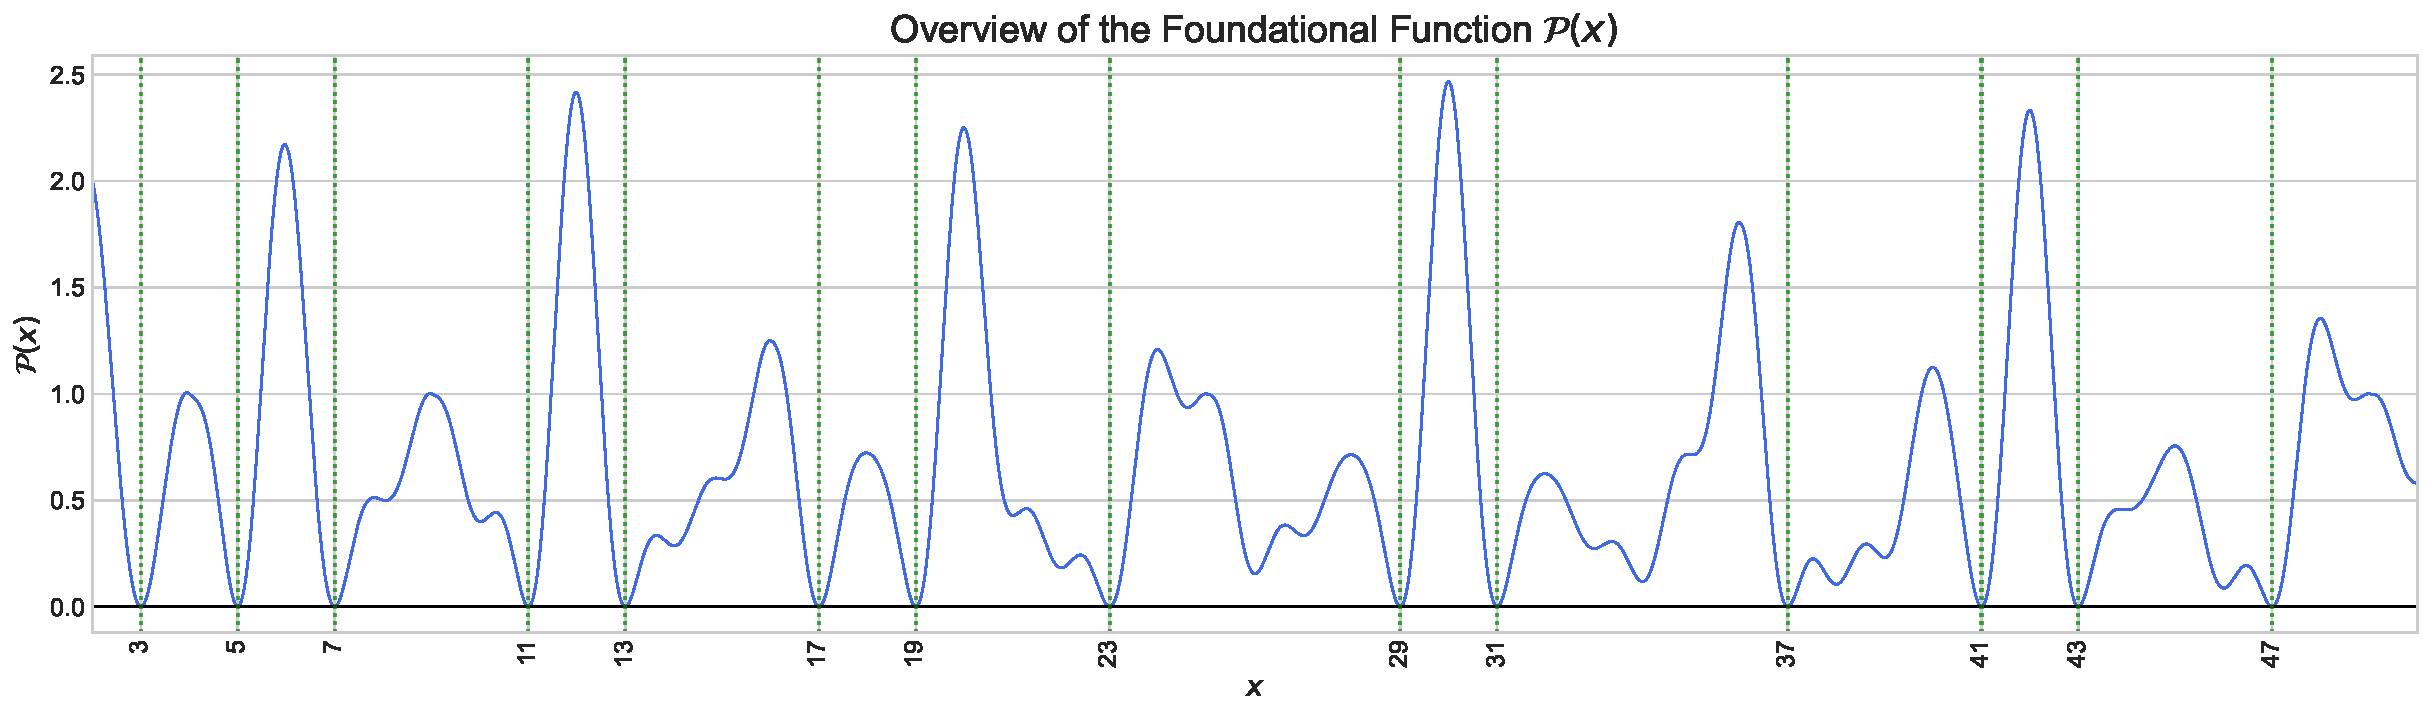
\includegraphics[width=\textwidth]{plot_overview.pdf}
\caption{Numerical profile of $\Px(x)$ for $2\le x\le 50$. Dotted vertical lines mark odd primes; $\Px(x)$ vanishes at these positions in accordance with Theorem~\ref{thm:primezero}.}
\label{fig:overview}
\end{figure}

\begin{figure}[!htbp]
\centering
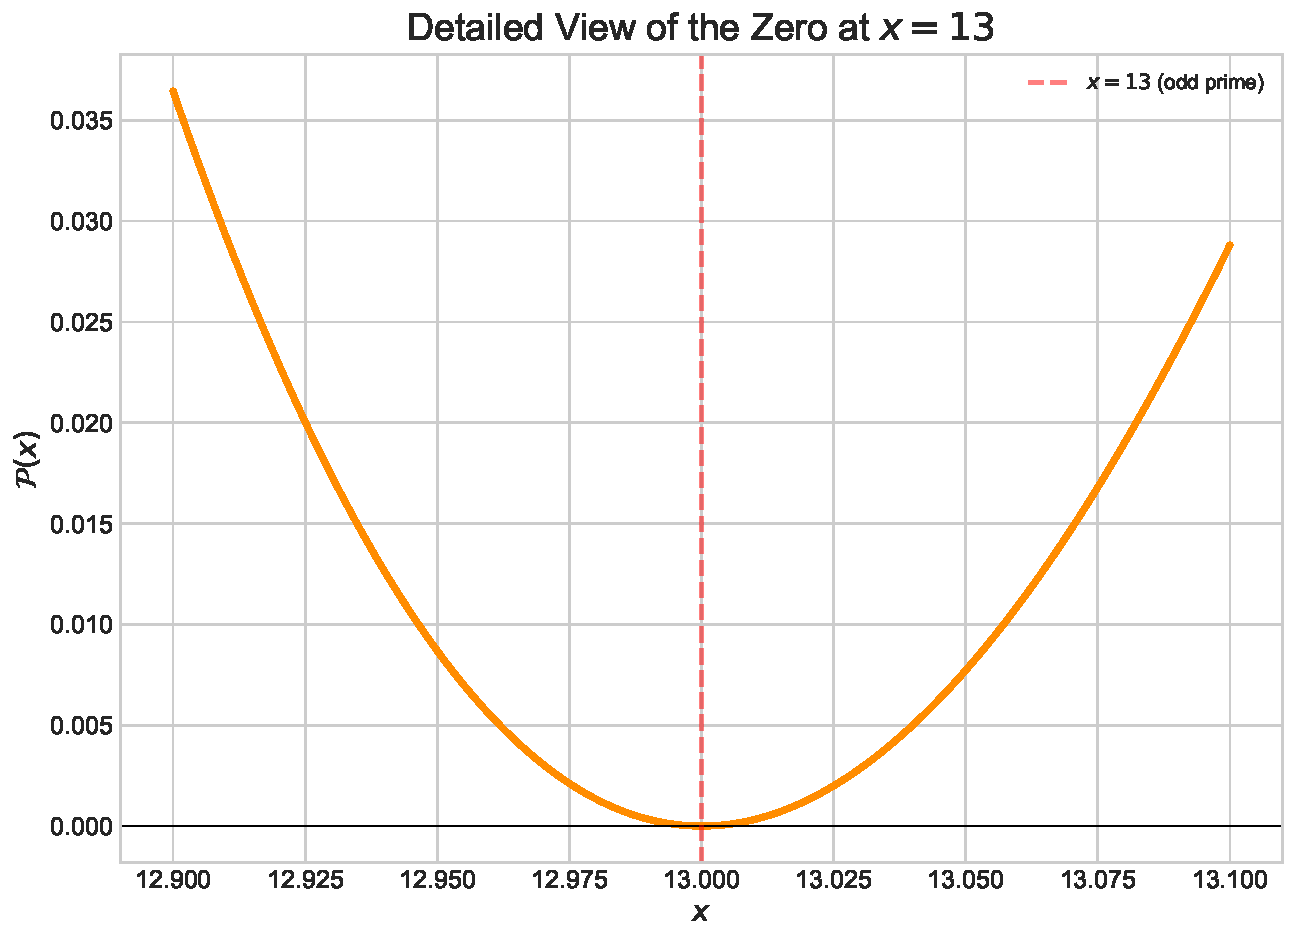
\includegraphics[width=0.8\textwidth]{plot_zoom_13.pdf}
\caption{Local behaviour of $\Px$ near $x=13$ (an odd prime). The zero crossing illustrates the proven prime–zero property.}
\label{fig:zoom13}
\end{figure}

% ---------------------------------------------------------------------------
\section{A $C^\infty$ Variant via Infinite Series Transformation}

\subsection{Motivation}
The function $\Px(x)$ achieves its property as a prime indicator at the cost of limited smoothness; the discontinuities in its second derivative are a direct result of the sharp cutoff in the summation limit $\lceil\sqrt{x}\rceil$. To create a globally smooth function suitable for broader analytic techniques, this sharp cutoff can be replaced with a smooth one, transforming the finite sum into a rapidly converging infinite series.

\subsection{Construction}
Let $\phi\colon[0, \infty) \to [0, 1]$ be a smooth ($C^\infty$) cutoff function with the following properties: $\phi(0)=1$, $\phi'(0)=0$, and $\phi(u)$ decays faster than any polynomial as $u\to\infty$ (superpolynomial decay). The conditions at $u=0$ ensure that $\Px_{\phi}(x)$ serves as a good approximation to $\Px(x)$ where the latter is defined. A function like $\phi(u) = e^{-u^4}$ is an excellent choice, as its higher-order derivatives at $u=0$ also vanish, making it very flat at the origin. A new function $\Px_{\phi}(x)$ is now defined.

\begin{definition}\label{def:Pphi}
For $x>1$ and a smooth cutoff function $\phi$ satisfying the conditions above, define
\begin{equation}\label{eq:Pphi}
\Px_{\phi}(x) = \frac{1}{x} \sum_{i=2}^{\infty} \phi\left(\frac{i}{\sqrt{x}}\right) F(x,i),
\end{equation}
where $F(x,i)$ is the Fejér kernel term from Definition~\ref{def:Px}. For $x\le1$, $\Px_{\phi}(x)$ is set to $0$.
\end{definition}
For any non-integer $x>0$, the terms $F(x,i)$ grow quadratically in $i$. The superpolynomial decay of the cutoff function $\phi$ ensures the absolute convergence of the series for all $x>0$, rendering the function $\Px_{\phi}(x)$ well-defined.

\subsection{Properties}
This new function $\Px_{\phi}(x)$ inherits the essential prime-indicator property of $\Px(x)$ while being significantly smoother.
\begin{property}[Preserved Prime-Zero Property]\label{prop:Pphizero}
For any smooth cutoff function $\phi$ satisfying $\phi(u)>0$ for all $u\in[0, \infty)$ and the decay conditions above, the function $\Px_{\phi}(x)$ has the property that for all real $x>2$,
\[
\Px_{\phi}(x)=0 \quad\Longleftrightarrow\quad x \text{ is an odd prime}.
\]
\end{property}
\begin{proof}
The logic follows that of Theorem~\ref{thm:primezero}.
\begin{enumerate}
    \item \textbf{Case 1: $x = p$ (odd prime).} For every $i\ge 2$, $i$ is not a divisor of $p$, so $F(p,i)=0$. The entire sum is a sum of zeros, hence $\Px_{\phi}(p)=0$.
    \item \textbf{Case 2: $x = n$ (composite).} Let $d$ be the smallest prime divisor of $n$, so $d\le\sqrt{n}$. The term for $i=d$ is $\frac{1}{n}\phi(\frac{d}{\sqrt{n}})F(n,d)$. As $F(n,d)=d^2 > 0$ and the cutoff factor $\phi(\frac{d}{\sqrt{n}})$ is strictly positive by definition of $\phi$, this term is strictly positive. All other terms in the sum are non-negative. Therefore, the total sum $\Px_{\phi}(n)>0$.
    \item \textbf{Case 3: $x$ is a non-integer.} $F(x,i) > 0$ for all $i$. Since $\phi$ is also strictly positive, every term in the sum is positive, and thus $\Px_{\phi}(x)>0$.
\end{enumerate}
The Prime-Zero Property is therefore preserved.
\end{proof}

\begin{property}[Global $C^\infty$-smoothness]\label{prop:Cinf}
The function $\Px_{\phi}(x)$ is of class $C^\infty$ for all $x>0$.
\end{property}
\begin{proof}
Let $g_i(x) = \frac{1}{x} \phi(i/\sqrt{x}) F(x,i)$ be the general term of the series. Each function $g_i(x)$ is of class $C^\infty$ for $x>0$ as a composition of smooth functions. To show that the sum $\Px_{\phi}(x) = \sum_{i=2}^{\infty} g_i(x)$ is also $C^\infty$, it is sufficient to show that for any integer $j \ge 0$, the series of derivatives $\sum_{i=2}^{\infty} g_i^{(j)}(x)$ converges uniformly on any compact interval $K \subset (0, \infty)$.
Let $K=[a,b]$ with $0 < a < b < \infty$.
The $j$-th derivative $g_i^{(j)}(x)$ can be determined using the general Leibniz rule on the product of three functions. The derivatives of $F(x,i)$ with respect to $x$ are bounded by a polynomial in $i$. For any integer $k \ge 0$, $|F^{(k)}(x,i)| \le C_k i^2$ for some constant $C_k$. The derivatives of $\frac{1}{x}$ are bounded on $K$. The derivatives of $\phi(i/\sqrt{x})$ introduce powers of $i$ and $x$ from the chain rule.
Applying the Leibniz rule, the $j$-th derivative $g_i^{(j)}(x)$ is a sum of terms, each a product of derivatives of the three factors. The $k$-th derivative of $\phi(u)$ with respect to $x$, where $u=i/\sqrt{x}$, introduces terms that are polynomial in $i$ and $x^{-1/2}$. Combined with the bounds on the derivatives of $F(x,i)$ and $1/x$, the term $g_i^{(j)}(x)$ is bounded on $K$ by a sum of terms of the form
\[ \left| \text{const} \cdot x^{-k_1} \cdot i^{k_2} \cdot \phi^{(m)}\left(\frac{i}{\sqrt{x}}\right) \cdot F^{(l)}(x,i) \right|, \]
where $m+l \le j$. For large $i$, this entire expression is bounded by a product of a polynomial in $i$ and terms involving $\phi$ and its derivatives:
\[ \sup_{x \in K} |g_i^{(j)}(x)| \le P_j(i) \cdot \sum_{m=0}^{j} \sup_{u \ge i/\sqrt{b}} |\phi^{(m)}(u)|, \]
where $P_j(i)$ is a polynomial in $i$ whose coefficients depend on $j$ and $K$.
By definition, the cutoff function $\phi$ and all its derivatives $\phi^{(m)}$ exhibit superpolynomial decay. This means that for any polynomial $P(u)$ and any integer $m \ge 0$, the product $P(u)\phi^{(m)}(u)$ tends to zero as $u \to \infty$. Consequently, the right-hand side of the inequality decays faster than any inverse polynomial in $i$. In particular, there exists a constant $C_j$ such that for all sufficiently large $i$:
\[ \sup_{x \in K} |g_i^{(j)}(x)| \le \frac{C_j}{i^2}. \]
Let $M_i = \sup_{x \in K} |g_i^{(j)}(x)|$. Since $\sum_{i=2}^{\infty} M_i$ converges by comparison with the p-series $\sum 1/i^2$, the Weierstrass M-test implies that the series of derivatives $\sum_{i=2}^{\infty} g_i^{(j)}(x)$ converges uniformly on $K$. A standard theorem from analysis states that if a series of functions $\sum g_i$ converges at a point and the series of derivatives $\sum g_i^{(j)}$ converges uniformly on a set, then the original series converges uniformly to a function $G$ and $G^{(j)} = \sum g_i^{(j)}$. Since this holds for any order $j \ge 0$, one can differentiate the series term-by-term to any order. Therefore, $\Px_{\phi}(x)$ is of class $C^\infty$ for all $x>0$.
\end{proof}

% ---------------------------------------------------------------------------
\section{Application: An Analytic Approximation for the Prime-Counting Function}

\subsection{Construction of an Approximating Function}
The prime-zero property of the function $\Px(x)$ allows for a formal construction of a function that approximates the prime-counting function $\pi(x)$. By definition, $\Px(n)$ is set to zero for $n \le 1$. The set of integers $n \ge 1$ for which $\Px(n)$ vanishes is therefore precisely $\{1\} \cup \{p \mid p \text{ is an odd prime}\}$.
The core idea is a sum of "soft indicator" terms that count 1 for a prime and nearly 0 for a composite number.

\begin{definition}[Approximation Formula]\label{def:pi_approx}
An analytic approximation for $\pi(x)$ is constructed as the sum
\begin{equation}\label{eq:pi_P_adaptive}
\pi_\Px(x; C) = \sum_{n=1}^{\lfloor x \rfloor} \left(1 - \frac{\Px(n)}{\Px(n) + C \cdot n^{-1}}\right),
\end{equation}
where $C$ is a small, positive constant (e.g., $C=0.0001$). The term $C \cdot n^{-1}$ serves as an adaptive threshold.
\end{definition}

In the sum, the term for $n=1$ contributes a value of 1 (since $\Px(1)=0$), which effectively accounts for the prime 2. Subsequent terms for $n>2$ contribute exactly 1 for odd primes (where $\Px(n)=0$) and a value slightly less than 1 for composites.

\subsection{Analysis of the Approximation Error}
A naive approach might use a small, constant threshold $\epsilon$ in the denominator. However, the lower bound of $\Px(n)$ for composite $n$ is not constant; it approaches zero as $n$ increases. Specifically, for composite numbers of the form $n=2p$ (where $p$ is a large prime), $\Px(n) = 2/p = 4/n$. A fixed $\epsilon$ would eventually be larger than $\Px(n)$, causing the indicator to fail. The use of an adaptive threshold $C \cdot n^{-1}$ circumvents this issue, as this term scales in the same way as the lower bound of $\Px(n)$.

\begin{property}[Bounded Term-wise Error]
For any composite integer $n \ge 4$, the contribution to the sum from the term corresponding to $n$, which represents the error for that term, is strictly positive and bounded by a constant that depends only on $C$.
Let $I(n; C) = 1 - \frac{\Px(n)}{\Px(n) + C \cdot n^{-1}}$ be the summand for $n$. For any prime $p$, $I(p; C) = 1$. For any composite $n$, the error $E(n) = I(n;C)$ is bounded.
\end{property}

\begin{proof}
For a composite number $n$, $\Px(n)>0$. The error term is:
\[ E(n) = 1 - \frac{\Px(n)}{\Px(n) + C/n} = 1 - \frac{1}{1 + \frac{C}{n \cdot \Px(n)}} \]
From the definition of $\Px(x)$, the identity $n \cdot \Px(n) = \sum_{d|n, 2\le d \le \sqrt{n}} d^2$ holds. Let this sum of divisor squares be denoted by $S_d(n)$. The error is thus:
\[ E(n) = 1 - \frac{1}{1 + \frac{C}{S_d(n)}} \]
The error $E(n)$ is maximized when the denominator $1 + \frac{C}{S_d(n)}$ is minimized. This occurs when $S_d(n)$ is at its minimum value.

For any composite number $n \ge 4$, there must be at least one prime factor $d \le \sqrt{n}$. The smallest possible such prime factor is 2. Therefore, the sum $S_d(n)$ is always greater than or equal to the square of the smallest possible prime factor.
\[ S_d(n) = \sum_{d|n, 2\le d \le \sqrt{n}} d^2 \ge 2^2 = 4. \]
This minimum value of $S_d(n)=4$ is attained for all numbers of the form $n=2p$ where $p$ is a prime such that $p>2$. The maximum possible error for any composite term, $E_{max}$, is therefore achieved when $S_d(n)=4$:
\[ E_{max} = 1 - \frac{1}{1 + \frac{C}{4}} = \frac{C/4}{1+C/4} = \frac{C}{4+C} \]
For any composite number $n$, the error $E(n)$ is bounded by $0 < E(n) \le E_{max}$. For instance, for a choice of $C=0.0001$, the maximum error for any single term is $E_{max} = 0.0001 / 4.0001 \approx 0.000025$. This proves that the error contribution of each composite number is strictly controlled.
\end{proof}

\begin{figure}[!htbp]
\centering
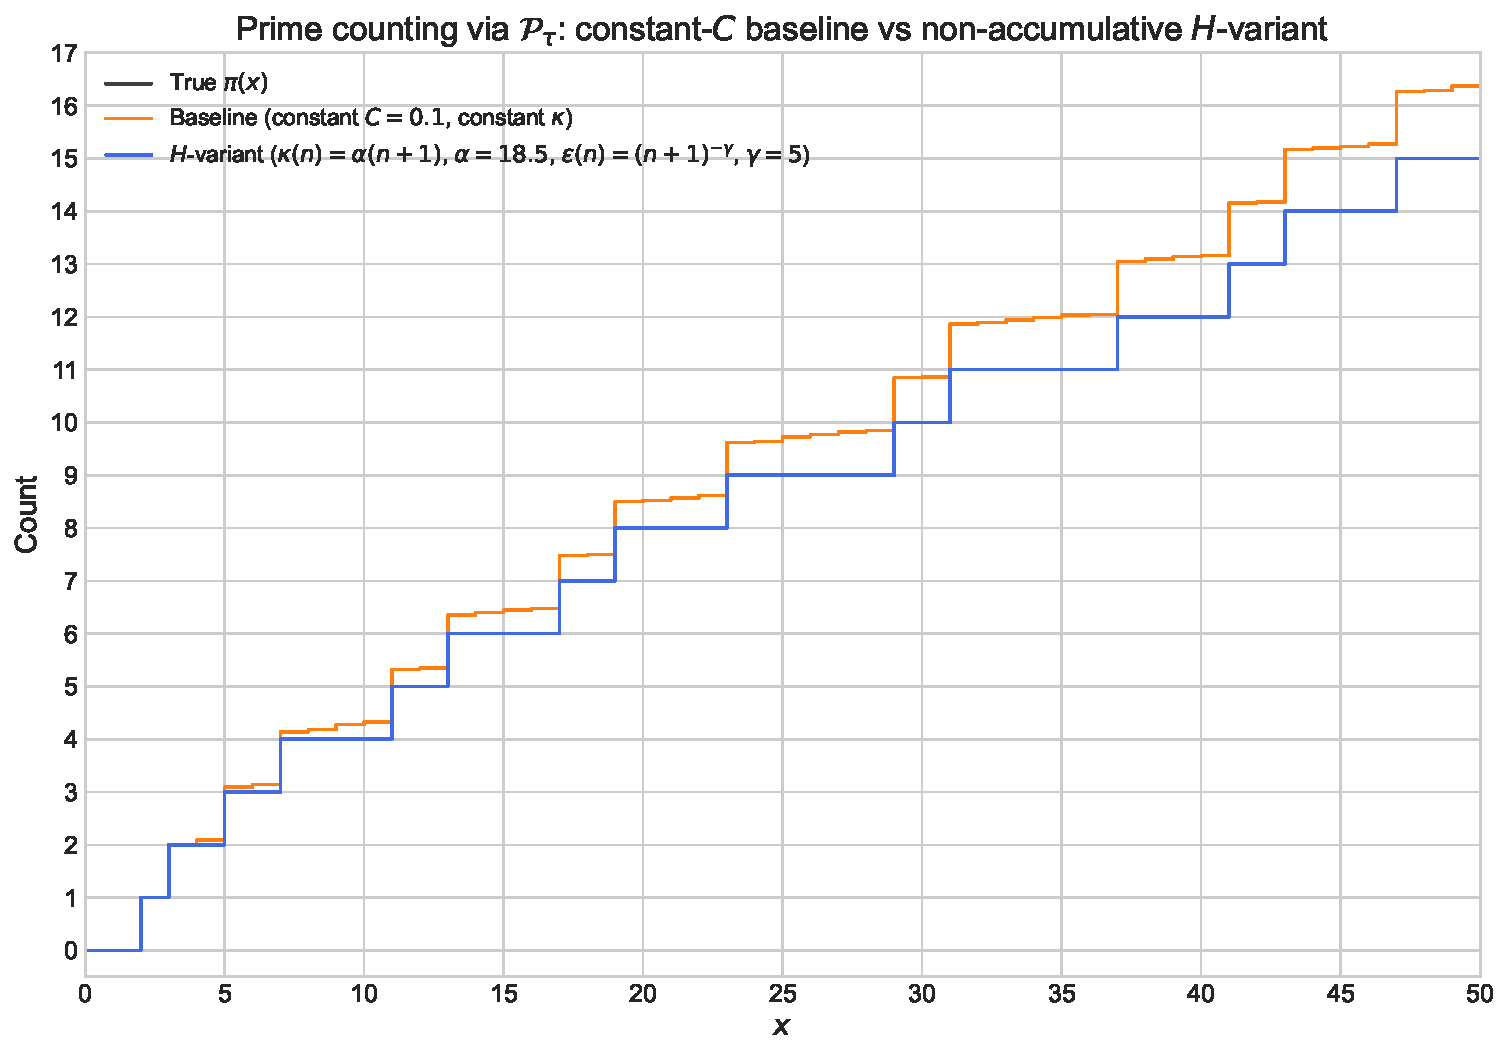
\includegraphics[width=\textwidth]{plot_prime_counting.pdf}
\caption{The step function $\pi_\Px(x)$ for $x\le 50$, constructed via the principles outlined. The steps of the function align with the prime numbers, illustrating the underlying prime-zero property of the function $\Px(x)$.}
\label{fig:primecounting}
\end{figure}

% ---------------------------------------------------------------------------
\section{Concluding Remarks}
The functions $\Px(x)$ and its smooth variant $\Px_{\phi}(x)$ offer a new perspective on prime-indicating functions, rooted in Fourier analysis. Their existence and properties open several avenues for further research. The existence of a $C^\infty$ function whose zeros are precisely the odd primes is of theoretical interest.
A primary open question concerns quantitative lower bounds, i.e., proving that $\Px_{\phi}(n) \ge c > 0$ for composite integers $n$ with an effective constant $c$.
A significant consequence of the function's properties is the construction of an analytic approximation for the prime-counting function $\pi(x)$ with a provably controlled error, as detailed in Section~6. The existence of such a direct link between a Fejér-kernel-based function and a controlled approximation of $\pi(x)$ underscores the theoretical potential of this approach.
The Python script (\texttt{numerical\_verification.py}) used for all numerical checks and plot generation is maintained in a public repository.%
\footnote{The repository is available at: \url{https://github.com/SebastianFoxxx/analytic-prime-indicator}}
Routines therein verify the prime-zero property and provide numerical evidence consistent with the claimed $C^\infty$-smoothness of the regularized function $\Px_{\phi}(x)$ at integer squares.
Further investigation into such questions could also include a comparative analysis of $\Px_{\phi}(x)$ with other recently proposed smooth prime indicators, such as the integral-based construction by Semenov~\cite{semenov2025}, and potential analogies to the explicit formulas of prime number theory~\cite{titchmarsh1986, montgomery2007, iwaniec2004, pimsCRG2024}.

% ---------------------------------------------------------------------------

\appendix
\section{Acknowledgements}
The author is grateful for the insightful discussions and steadfast support provided by friends, family, and colleagues, which were invaluable during the development of this work.

\begin{thebibliography}{13}

\bibitem{pimsCRG2024}
L.~Bellaïche, S.~J.~Lester, and A.~T.~M.~Anisha, \emph{Open Problems in Comparative Prime Number Theory}, arXiv:2407.03530 [math.NT], 2024.

\bibitem{hardy2008}
G.\,H.~Hardy and E.\,M.~Wright, \emph{An Introduction to the Theory of Numbers}, 6th ed., Oxford University Press, 2008.

\bibitem{helfgott2023}
A.~Helfgott, Analytic prime indicators revisited, \emph{Proc.\ Lond.\ Math.\ Soc.} \textbf{127} (2023), 1–29.
\bibitem{hiary2018}
G.\,B.~Hiary and N.~Hiary, An explicit prime-detecting function, \emph{J.\ Théor.\ Nombres Bordeaux} \textbf{30} (2018), 105–132.
\bibitem{iwaniec2004}
H.~Iwaniec and E.~Kowalski, \emph{Analytic Number Theory}, AMS Colloquium Publ.\ 53, 2004.

\bibitem{mazzanti2024}
S.~Mazzanti, On arithmetic terms expressing the prime-counting function and the n-th prime, \emph{arXiv:2412.14594 [math.NT]}, 2024.

\bibitem{mills1947}
W.\,H.~Mills, A prime-representing function, \emph{Bull.\ Amer.\ Math.\ Soc.} \textbf{53} (1947), 604.

\bibitem{montgomery2007}
H.\,L.~Montgomery and R.\,C.~Vaughan, \emph{Multiplicative Number Theory I: Classical Theory}, Cambridge University Press, 2007.

\bibitem{semenov2025}
S.~Semenov, A Smooth Analytical Approximation of the Prime Characteristic Function, \emph{arXiv:2504.14414 [math.GM]}, 2025.

\bibitem{seriprim2022}
E.~Seri, On analytic prime indicators, \emph{J.\ Number Theory} \textbf{162} (2022), 287–303.
\bibitem{titchmarsh1986}
E.\,C.~Titchmarsh, \emph{The Theory of the Riemann Zeta-Function}, 2nd ed., rev. by D. R. Heath-Brown, Oxford University Press, 1986.

\bibitem{willans1964}
C.\,P.~Willans, On formulae for the $n$-th prime number, \emph{Math.\ Gazette} \textbf{48} (1964), 413–415.
\bibitem{zygmund2002}
A.~Zygmund, \emph{Trigonometric Series}, 3rd ed., Cambridge Univ.\ Press, 2002.

\end{thebibliography}

\end{document}